\chapter{Agente Inteligentes}

Agentes autónomos trabajan para resolver problemas en un entorno dinámico y complejo. \ul{Un agente es un sistema computacional que opera en un entorno y es capaz de percibirlo y actuar sobre él}. Un agente inteligente es aquel que actúa de manera racional, es decir, que actúa para alcanzar sus objetivos, basándose en la información que percibe y en su conocimiento del entorno.
Más formalmente,
\begin{definition}
   [Wooldrdige]
   Un agente es un sistema informático
   capaz de actuar autónomamente en algún
   entorno con el fin de alcanzar los objetivos
   que se le han delegado.
\end{definition}

\begin{definition}
   [Wooldridge updated]
   Cualquier proceso computacional dirigido por el objetivo capaz
   de interaccionar con su entorno de forma \textbf{flexible} (Reactivo, Proactivo, Social) y \textbf{robusta}
\end{definition}

\begin{figure}[htbp]
   \centering
   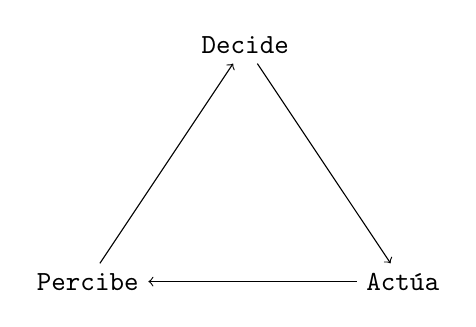
\begin{tikzpicture}
      \node (percibe) at (0, 0) {\texttt{Percibe}};
      \node (decide) at (2, 3) {\texttt{Decide}};
      \node (actua) at (4, 0) {\texttt{Actúa}};

      \draw[->] (percibe) -- (decide);
      \draw[->] (decide) -- (actua);
      \draw[->] (actua) -- (percibe);
   \end{tikzpicture}

   \caption{Agente bucle}
   \label{fig:agenteBucle}
\end{figure}

Un agente reactivo reacciona a los cambios del entorno. No tiene que ser el más rápido, pero la reacción debe ser útil. Un agente proactivo actúa para alcanzar sus objetivos, planifica y actúa en consecuencia. Un agente social interactúa con otros agentes.

En entornos complejos, un agente no tiene control completo sobre su entorno, sólo tiene un control parcial. Control parcial significa que el agente puede influir sobre el entorno con sus acciones. Una acción ejecutada por un agente puede fallar o tener el efecto deseado. En conclusión, los entornos son no deterministas y los agentes deben estar preparados para posibles fallos.

\begin{itemize}
   \item Accesible vs inaccesible.\\
   Un entorno accesible es aquel en el que el agente puede
   obtener información completa, exacta y actualizada del
   estado del entorno.
   \item Determinista vs no determinista.\\
   Un entorno determinista es aquel en el que cualquier
   acción tiene un único efecto garantizado, no hay
   incertidumbre sobre el estado resultante de la ejecución de
   una acción\\
   El mundo físico puede a todos los efectos ser
   considerado como no determinista.\\
   Los entornos no deterministas presentan grandes
   problemas para el diseñador de agentes.
   \item Episódico vs no episódico\\
   En un entorno episódico el desempeño/actuación de un
   agente depende de un número discreto de episodios, no
   existiendo enlaces (relación) entre el desempeño de un agente
   en escenarios distintos.
   Los entornos episódicos son, desde el punto de vista del
   desarrollador de agentes, más sencillos porque el agente puede
   decidir que acción ejecutar basándose únicamente en el
   episodio actual, no necesita razonar sobre las interacciones
   entre el episodio actual y los episodios futuros.
   \item Estático vs dinámico\\
   Un entorno estático es aquel en el que se puede asumir que
   no se producen cambios excepto los provocados por la
   ejecución de acciones del agente.
   Un entorno dinámico es aquel que tiene otros procesos que
   operan en el, y que por lo tanto se producen cambios que están
   fuera del control del agente.
   \item Discreto vs continuo\\
   Un entorno es discreto si en él hay un número fijo y finito de
   acciones y percepciones.
   El juego del ajedrez es un ejemplo de entorno discreto, y la
   conducción de un taxi un ejemplo de entorno continuo (AIMA,
   Russell and Norvig).
\end{itemize}

Asumimos que el entorno puede estar en uno cualquiera de los
estados de un conjunto finito de estados instantáneos discreto
(E):
\begin{equation}
   E = { s_1,s_2,...}
\end{equation}
• Se asume que los agentes tienen disponible un repertorio
(conjunto finito) de posibles acciones que transforman el
estado del entorno :
\begin{equation}
   Ac = { \alpha_1,\alpha_2,...}
\end{equation}

\begin{align}
   \textit{Acción} & : E \rightarrow A \\
   \textit{Percibir} & : E \rightarrow P\\
   \textit{Decisión} & : P^* \rightarrow A\\
   \textit{Selección} & : I \rightarrow Ac \\
   \textit{actualizar\_estados} & : I \times P \rightarrow I\\
   \textit{actualizar\_objetivos} & : G \times P \rightarrow G \\
   \textit{Acción (update)} & : I \times G \rightarrow Ac
\end{align}
\text{La acción dependerá del estado interno y de los objetivos que el agente quierá alcanzar}
\note{
   \begin{itemize}
      \item 
      $P$ es un conjunto (no vacío) de percepciones (entradadas perceptivas), que relaciona estados del entorno con percepciones
      \item $I$ es el conjunto de todos los estados internos del agente
      \item $G$ es el conjunto de todos los objetivos del agente
   \end{itemize}
}

\section{Jason}

Jason es un lenguaje de programación basado en agentes, que permite la programación de agentes inteligentes. Jason es un lenguaje de alto nivel, basado en la lógica, que permite la programación de agentes inteligentes, y es una extension de AgentSpeak.

{Los elementos fundamentales del Lenguaje son:\ns
\begin{itemize}
	\item \textbf{Creencias} (Beliefs)
	\item \textbf{Objetivos} (Goals)
	\item \textbf{Planes} (Plans, Intentions)
\end{itemize} }


\subsection{Creencias}
{Cada agente tiene una base de \textbf{creencias}, colección de literales representados como \textit{predicados}.\ns
\begin{itemize}
	\item \lstinline|tall(jhon).|
	\item \lstinline|likes(jhon, music)|
\end{itemize}}
\textbf{Anotaciones} son detalles asociados a una creencia.\\\lstinline|busy(jhon)[expires(autum)]|
Las anotaciones aportan ``elegancia'' al lenguaje y facilitan el manejo de la base de creencias.\\
Existen anotaciones que tienen un signicado especial para el
interprete. En particular la anotacion \lstinline|source|.

Hay tres tipos de fuentes de informacion para los agentes
\begin{itemize}
	\item \textit{Informacion perceptual}: aquella que percibe del entorno
	      \begin{itemize}
		      \item \lstinline|source(percept)|
		      \item \lstinline|(colour(box1,blue)[source(percept)])|
	      \end{itemize}
	\item \textit{Comunicacion}: aquella que proviene de otro agente del
	      sistema
	      \begin{itemize}
		      \item \lstinline|source(id agente)|
		      \item \lstinline|(colour(box1,blue)[source(bob)])|
	      \end{itemize}
	\item \textit{Notas mentales}: creencias que provienen del propio agente
	      \begin{itemize}
		      \item \lstinline|source(self)|
		      \item \lstinline|(colour(box1,blue)[source(Self)])|
	      \end{itemize}
\end{itemize}

\subsection{Objetivos}

{Existen dos tipos de objetivos en Jason:\ns
\begin{enumerate}
	\item \textbf{Achievement goals}(operador \lstinline|!|): Expresan un estado del
mundo que el agente desea conseguir.
   \begin{itemize}
      \item \lstinline|own(house)|
   \end{itemize}
	\item \textbf{Test goals}(operador \lstinline|?|): Usados normalmente para recuperar información de la base de creencias.
   \begin{itemize}
      \item \lstinline|bank_balance(BB)|
   \end{itemize}
\end{enumerate}
}
\subsection{Planes}
{Un plan tiene tres partes\ns
\begin{itemize}
	\item \textbf{Triggering event}: Cambios en las creencias o objetivos del agente
	\item \textbf{Context}: Determinan si un plan es aplicable. Literales que deben ser una consecuencia lógica de
   la base de creencias para que el plan se instancie.
	\item \textbf{Body}: Sucesión de acciones que comporta el plan. Es una secuencia de acciones. Pueden existir nuevos subobjetivos.
\end{itemize}}


\begin{figure}[htbp]
   \centering
   \begin{tikzpicture}[
      every node/.style={draw, minimum height=1cm, anchor=west},
      event/.style={fill=white},
      context/.style={fill=white},
      body/.style={fill=white},
      label/.style={anchor=north}
      ]
      
      % Nodes
      \node[event] (event) {\lstinline|+!prepare(Something)|};
      \node[context, right=0cm of event] (context) { \lstinline| NoOfPeople(N) & stock(Something,S) & S > N <-|};
      \node[body, right=0cm of context] (body) {.\hspace{3em}\lstinline|.......|\hspace{3em}.};
      
      % Labels
      \node[label, below=0.5cm of event] {Evento Disparador};
      \node[label, below=0.5cm of context] {Contexto};
      \node[label, below=0.5cm of body] {Cuerpo};
      
      % Outline for grouping
      \draw [thick] (event.north west) -- (event.south west) -- (body.south east) -- (body.north east) -- (event.north west);
      
   \end{tikzpicture}
   
   \caption{Plan schema}
   \label{fig:planschema}
\end{figure}

\subsubsection{Cuerpo de un plan}

El cuerpo del plan es secuencia de instrucciones separadas por ``\lstinline|;|''. Estas instrucciones pueden ser:\ns
\begin{itemize}
	\item Actions: Acciones externas que se denotan por un predicado.
	      Proporcionan un ``feedback''.
	      \begin{lstlisting}
   rotate(leftarm, 45)
         \end{lstlisting}
	\item Achievement goals: subobjetivos que deben ser alcanzados para que el
	      plan continúe su ejecución (si en lugar de emplear ``\lstinline|!|'' se emplea ``\lstinline|!!'|', el
	      plan no suspenderá su ejecución).
	      \begin{lstlisting}
	!!at(home); call(john) en lugar de !at(home); call(john).
         \end{lstlisting}
	\item Test goals: Para recuperar información de la BB o verificar si el agente
	      cree algo.
	      \begin{lstlisting}
	?coords(Tarjet,X,Y).
         \end{lstlisting}
   \item \textbf{Mental Notes}: Anotación source(self). Sirven para añadir, modificar o eliminar nuevas
   creencias.
   \begin{lstlisting}
      +currenttargets(NumTargets); [Se anade]
      -+currenttargets(NumTargets); [Se modifica]
   \end{lstlisting}
   \item \textbf{InternalActions}: Son acciones que no modifican el entorno. Se diferencian de acciones del
   entorno por el carácter ``\lstinline|.|''.
   \begin{lstlisting}
      .print(...); .send(...);
   \end{lstlisting}
   \item \textbf{Expressions}: Su sintaxis es semejante a la de Prolog.
   \begin{lstlisting}
      X >=Y*2
   \end{lstlisting}
   \item \textbf{Plan Labels}: Los planes pueden estar etiquetados
   \begin{lstlisting}
      @labelte: ctxt<-body.
   \end{lstlisting}
\end{itemize}

\subsubsection{Fallo de un Plan}
\begin{itemize}
	\item Un plan puede fallar por tres causas principales:
   \begin{itemize}
   	\item Falta de planes relevantes o aplicables para un ``achievement goal''
	\item Fallo de un ``test goal''
	\item Fallo de una acción
   \end{itemize}
	\item Cuando un plan falla se genera un evento \lstinline|-!g| (goal deletion event) si se generó por la adición de un ``achievement goal'' o ``test goal''.
	\item El plan que se dispare por el fallo se añade a la pila de intenciones del plan que ha fallado.
\end{itemize}

\subsection{Ejemplos}


\lstset{language=Java}
\begin{lstlisting}
   /* Creencias iniciales */
   inicio.
   /* Planes */
   +inicio <- .print("Hola Mundo"). //plan que se dispara al inicio
\end{lstlisting}

\begin{lstlisting}
   /* Creencias iniciales */
   fact(0,1).
   /* Planes */
   +fact(X,Y) : X < 5
   <- +fact(X+1, (X+1) * Y ).
   +fact(X,Y) : X = 5
   <- .print("fact 5 == ", Y ).
\end{lstlisting}

\begin{lstlisting}
   /* Objetivos iniciales */
   !dots.
   !control.
   /* Planes */
   +!dots
   <- .print("."); // imprime puntos en un bucle sin fin
   !!dots.
   +!control
   <- .wait(30); // este plan es un bucle que activa y desactiva el otro plan
   .suspend(dots); // suspende la intencion asociada al plan dots
   .println;
   .wait(200);
   .resume(dots); // reactiva la intencion asociada al plan dots
   !!control
\end{lstlisting}

\begin{lstlisting}
   // Un agente que soluciona el problema del mundo de bloques
   /* Creencias iniciales y reglas */
   clear(table).
   clear(X) :- not(on(_,X)). // la creencia clear(X) es cierta cuando no tiene nada encima
   tower([X]) :- on(X,table). // la torre X es cierta cuando X esta sobre la mesa
   // X puede ser un bloque o varios
   tower([X,Y|T]) :- on(X,Y) & tower([Y|T]).
   // la torre va creciendo si un bloque X se pone sobre el bloque Y
   /* Objetivos iniciales */
   // Marca el estado final a alcanzar
   !state([[a,e,b],[f,d,c],[g]]).

   /* Planes */
   // Alcanzar una torre
   +!state([]) <- .print("Finalizado!").
   +!state([H|T]) <- !tower(H); !state(T).
   // Alcanzar un estado donde la torre esta construida
   +!tower(T) : tower(T). // La torre deseada ya existe, no hay nada que hacer
   +!tower([T]) <- !on(T,table). // La torre es de un solo elemento
   +!tower([X,Y|T]) <- !tower([Y|T]); !on(X,Y). // divido el problema en subproblemas
\end{lstlisting}